% To je predloga za poročila o domačih nalogah pri predmetih, katerih
% nosilec je Blaž Zupan. Seveda lahko tudi dodaš kakšen nov, zanimiv
% in uporaben element, ki ga v tej predlogi (še) ni. Več o LaTeX-u izveš na
% spletu, na primer na http://tobi.oetiker.ch/lshort/lshort.pdf.
%
% To predlogo lahko spremeniš v PDF dokument s pomočjo programa
% pdflatex, ki je del standardne instalacije LaTeX programov.

\documentclass[a4paper,11pt]{article}
\usepackage{a4wide}
\usepackage{fullpage}
\usepackage[utf8x]{inputenc}
\usepackage[slovene]{babel}
\selectlanguage{slovene}
\usepackage[toc,page]{appendix}
\usepackage[pdftex]{graphicx} % za slike
\usepackage{setspace}
\usepackage{color}
\definecolor{light-gray}{gray}{0.95}
\usepackage{listings} % za vključevanje kode
\usepackage{hyperref}
\renewcommand{\baselinestretch}{1.2} % za boljšo berljivost večji razmak
\renewcommand{\appendixpagename}{Priloge}

\lstset{ % nastavitve za izpis kode, sem lahko tudi kaj dodaš/spremeniš
language=Python,
basicstyle=\footnotesize,
basicstyle=\ttfamily\footnotesize\setstretch{1},
backgroundcolor=\color{light-gray},
}

\title{Risanje sinusoid}
\author{David Rubin (david.rubin@student.um.si)}
\date{\today}

\begin{document}

\maketitle

\section{Uvod}

V programskem orodju  Octave ali Python izdelajte program,, ki omogoča prikaz sinusoide s poljubno frekvenco, amplitudo in fazo, in sicer na poljubnem časovnem intervalu in s poljubno frekvenco vzorčenja. Vsi ti parametri naj bodo interaktivno nastavljivi preko grafičnega vmesnika. 

Odgovorite na naslednja vprašanja:
\begin{enumerate}
	\item Pri katerih vzorčevalnih frekvencah se izbrana sinusoida ne prikaže pravilno in katera izmed njenih lastnosti (amplituda, frekvenca, faza) se pri tem spremeni ter kako (t.j. kako se spremeni amplituda, kako faza in kako frekvenca prikazane sinusoide)?
 	\item Se je ob tem spremenila dejanska sinusoida ali le njen prikaz? Kaj to pomeni za analizo digitalnih signalov?
	\item Kako pa se s frekvenco vzorčenja spremenijo amplituda, faza in frekvenca sinusoide, če uporabimo analitičen zapis sinusoide, torej če sinusoido zapišemo s kompleksnimi števili: $s(t) = A\cdot \sin(2\pi \cdot f \cdot t + \varphi) + j \cdot A \cdot \cos(2 \pi \cdot f + \varphi)$, kjer je $A$ amplituda, $f$ frekvenca in $\varphi$ faza, $j$ pa je imaginarna enota ($\sqrt{-1}$)?
	\item Kaj smo torej pridobili z analitičnim zapisom sinusoide in kaj smo za to žrtvovali?


\end{enumerate}

\section{Poročilo}

Rešitev sem implementiral kot Python program (za delovanje potrebuje PyQt5, matplotlib in numpy), ki je priložen poročilu (\textit{sinus.py}).

\begin{enumerate}
	\item\textbf{ Pri katerih vzorčevalnih frekvencah se izbrana sinusoida ne prikaže pravilno in katera izmed njenih lastnosti (amplituda, frekvenca, faza) se pri tem spremeni ter kako (t.j. kako se spremeni amplituda, kako faza in kako frekvenca prikazane sinusoide)?}

		V kolikor smo signal vzorčili s frekvenco, ki je nižja od $2 \cdot f$, se nam pojavijo tako imenovane alias frekvence. Točke pri vzorčenju nam pri prenizki vzorčevalni frekvenci ($f_s < 2 \cdot f$) sovpdajeo s sinusoidami nižjih frekvenc. Amplituda se načeloma ne spremeni (v kolikor jo znamo iz realnega grafa pravilno prebrati), spremenita se pa frekvenca, saj je sedaj v signalu poleg dejanske prisotna tudi nižja, ki ima lahko tudi različno fazo od prvotne (glej sliko~\ref{slika1}).	
	\begin{figure}[htbp]
	\begin{center}
	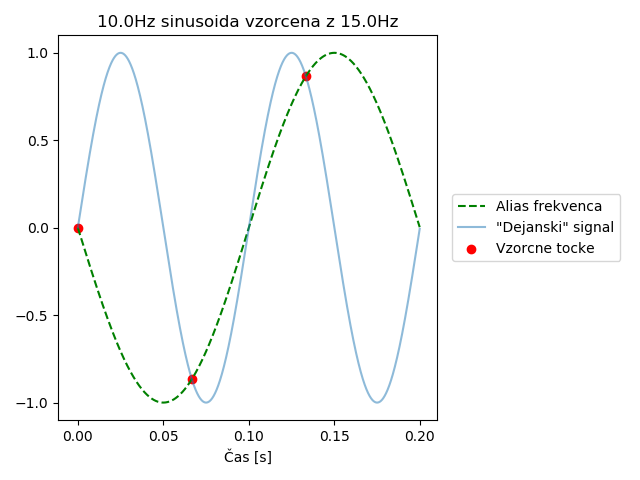
\includegraphics[scale=0.6]{alias.png}
	\caption{Pojavitev nižje frekvence pri nezadostno visoki frekvenci vzorčenja.}
	\label{slika1}
	\end{center}
	\end{figure}


 	\item \textbf{Se je ob tem spremenila dejanska sinusoida ali le njen prikaz? Kaj to pomeni za analizo digitalnih signalov?}

	Ob tem pojavu se dejanska sinusoida ne spremeni. Zaradi ``slabega'' vzorčenja, ki smo ga izvajali pa smo popačili našo predstavitev tega signala. V kolikor te popačene podatke uporabimo za analizo prvotnega signala (ali pa ga poskušamo rekonstruirati) bomo dobili slabe rezultate. S prenizko vzorčevalno frekvenco nismo samo izgubili del podatkov, ampak smo v signal vnesli tudi \textit{aliasing} in si popačili preostali signal.

 	
	\item \textbf{Kako pa se s frekvenco vzorčenja spremenijo amplituda, faza in frekvenca sinusoide, če uporabimo analitičen zapis sinusoide, torej če sinusoido zapišemo s kompleksnimi števili: $s(t) = A\cdot \sin(2\pi \cdot f \cdot t + \varphi) + j \cdot A \cdot \cos(2 \pi \cdot f + \varphi)$, kjer je $A$ amplituda, $f$ frekvenca in $\varphi$ faza, $j$ pa je imaginarna enota ($\sqrt{-1}$)?}
	
	
	\item \textbf{Kaj smo torej pridobili z analitičnim zapisom sinusoide in kaj smo za to žrtvovali?}
	
	Z analitičnim zapisom smo veliko bolje predstavili našo sinusoido, saj je trivialno razbrati amplitudo in fazo podanega signala. Pri tem pa smo porabili $2\times$ več prostora za opis krivulje.

\end{enumerate}

\end{document}
